
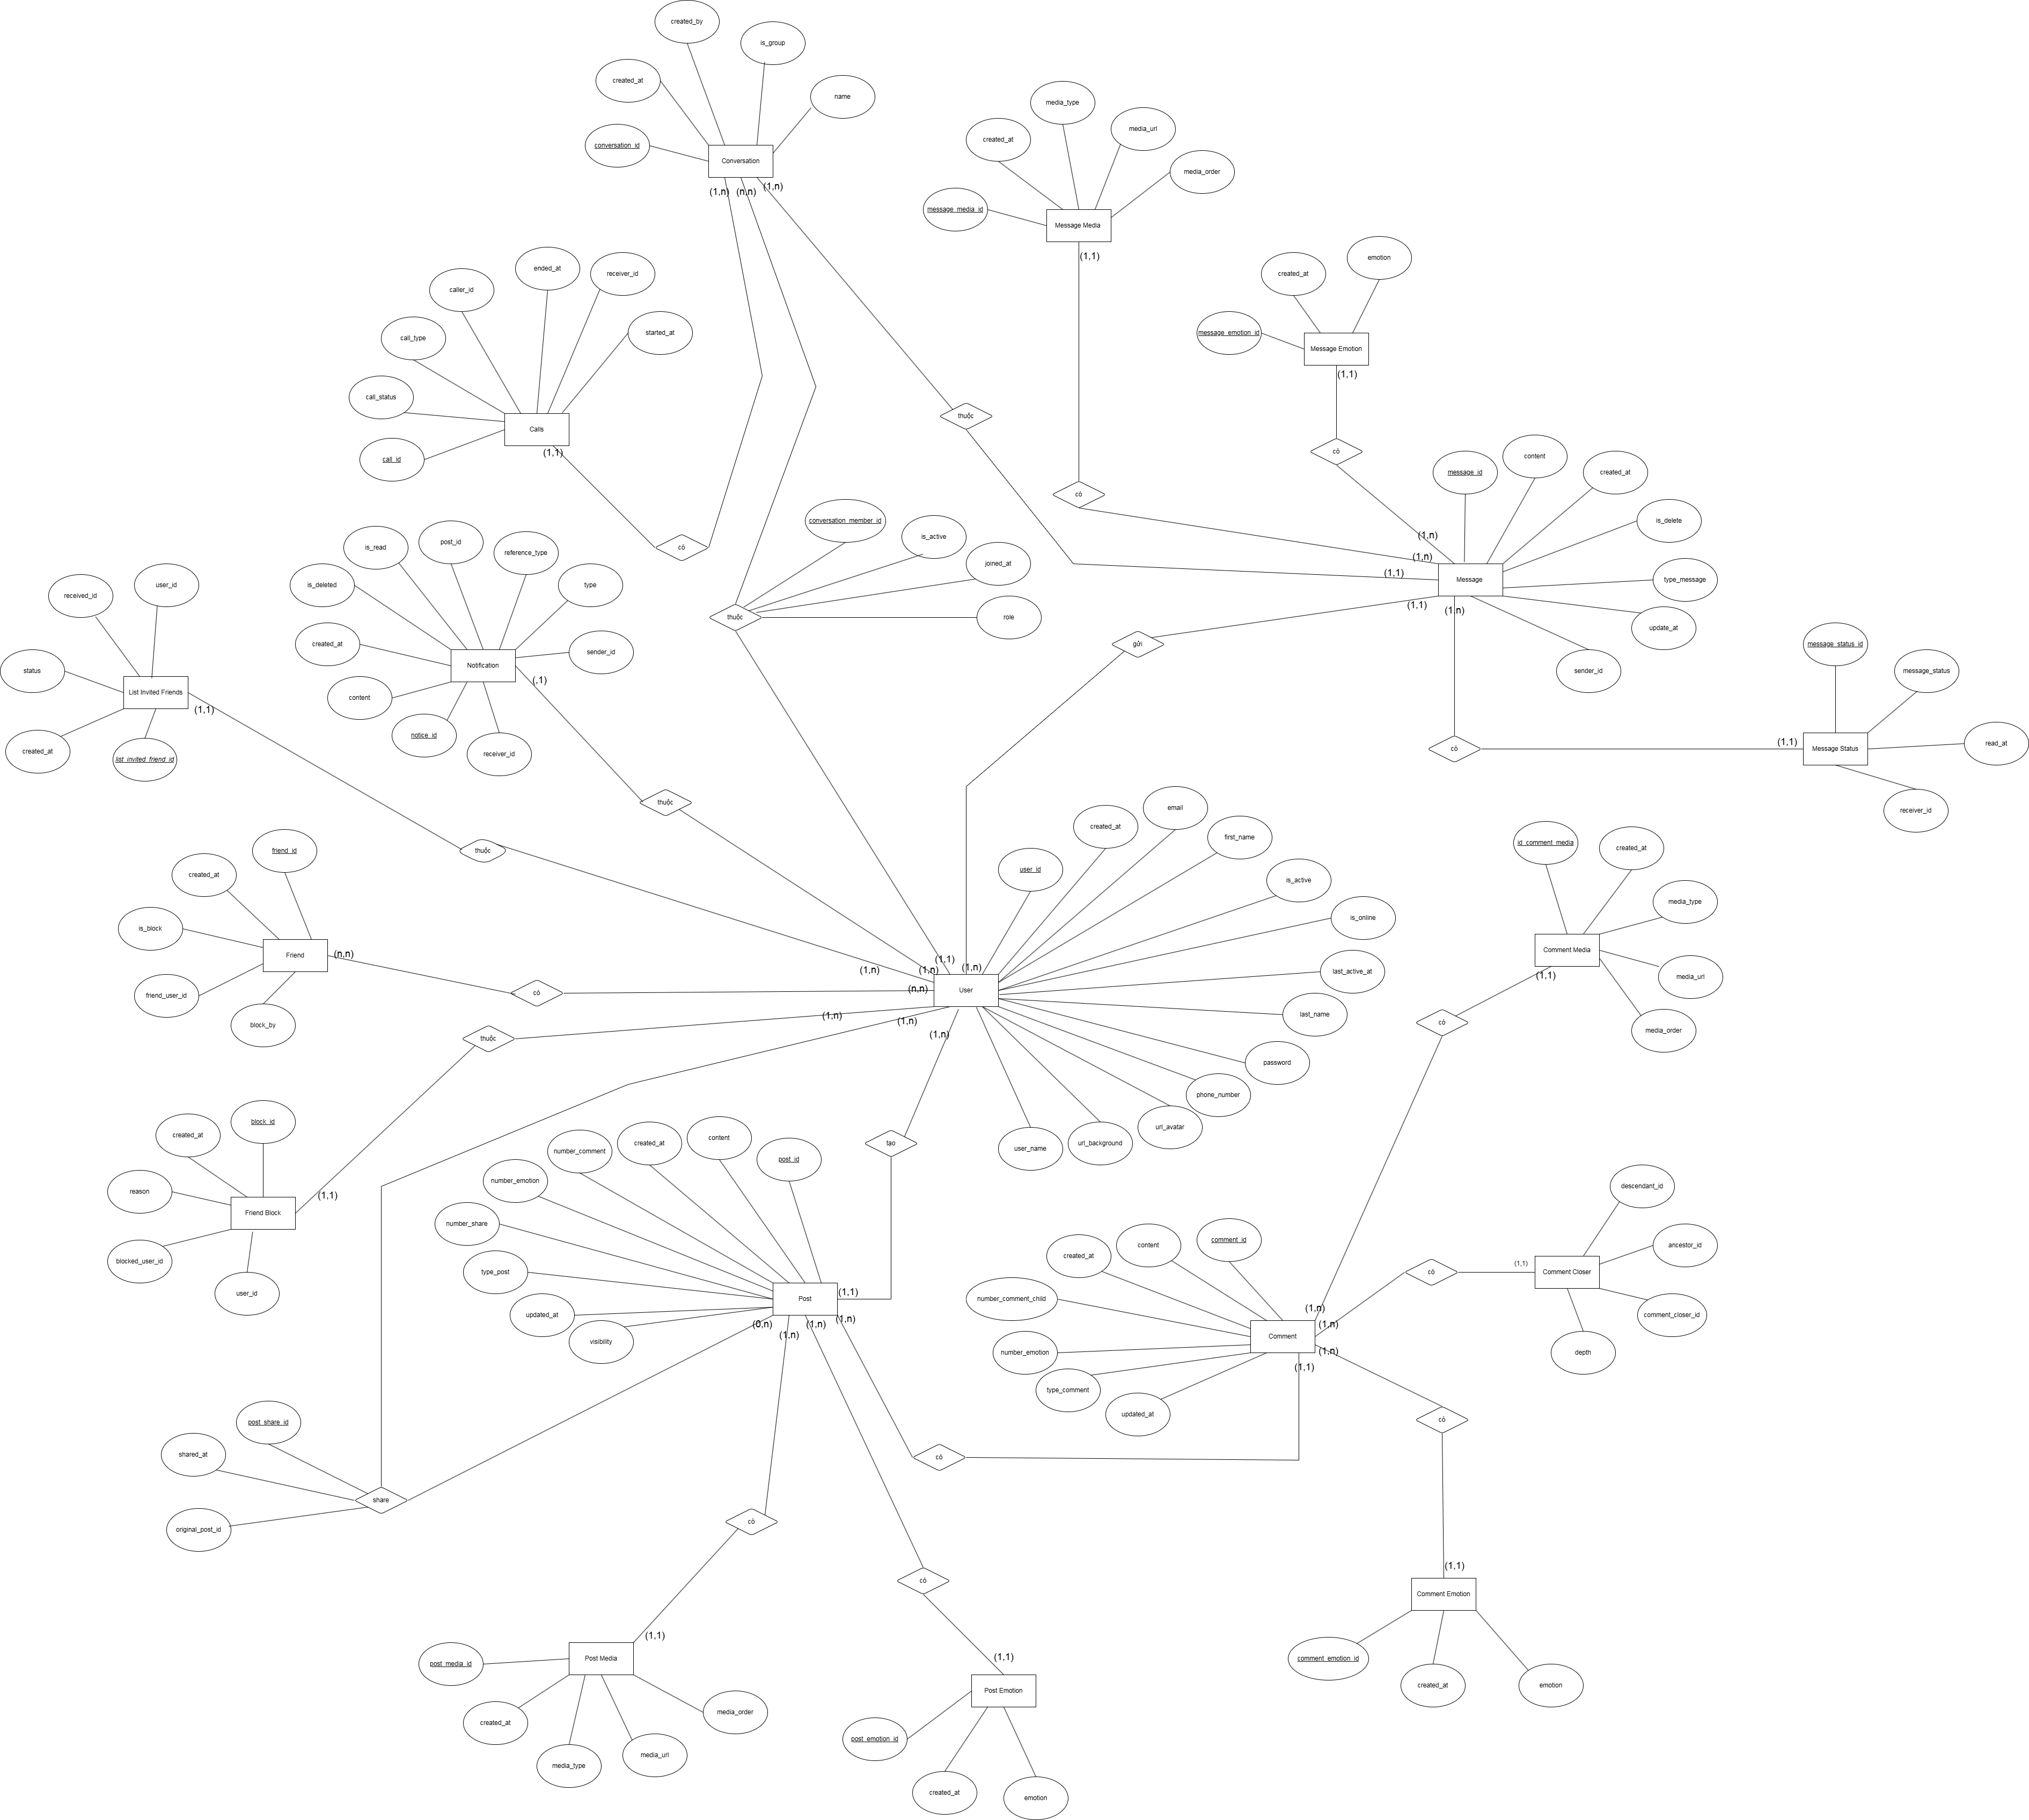
\includegraphics[width=\textwidth]{img/ERD_Instagram.png}

\section{Entity \texttt{User}}

\begin{longtable}{|>{\raggedright\arraybackslash}p{4cm}|>{\raggedright\arraybackslash}p{4cm}|>{\raggedright\arraybackslash}p{6cm}|}
\hline
\textbf{Tên thuộc tính} & \textbf{Kiểu dữ liệu} & \textbf{Mô tả} \\
\hline
\texttt{userId} & \texttt{int} & Khóa chính, tự động tăng \\
\hline
\texttt{userName} & \texttt{String} & Tên đăng nhập (không trùng) \\
\hline
\texttt{firstName} & \texttt{String} & Tên \\
\hline
\texttt{lastName} & \texttt{String} & Họ \\ 
\hline
\texttt{email} & \texttt{String} & Email (không trùng) \\
\hline
\texttt{password} & \texttt{String} & Mật khẩu đã mã hóa \\
\hline
\texttt{phoneNumber} & \texttt{String} & Số điện thoại \\
\hline
\texttt{isActive} & \texttt{Boolean} & Trạng thái hoạt động \\
\hline
\texttt{lastActiveAt} & \texttt{LocalDateTime} & Thời gian hoạt động gần nhất \\
\hline
\texttt{createdAt} & \texttt{LocalDateTime} & Thời điểm tạo tài khoản \\
\hline
\texttt{isOnline} & \texttt{Boolean} & Đang online hay không \\
\hline
\texttt{urlAvatar} & \texttt{String} & URL ảnh đại diện \\
\hline
\texttt{urlBackground} & \texttt{String} & URL ảnh nền \\
\hline
\end{longtable}

\vspace{0.5cm}
Mối quan hệ:
\begin{itemize}
    \item \textbf{User} có nhiều \textbf{ConversationMember}.
    \item \textbf{User} có nhiều \textbf{Role} (ManyToMany).
\end{itemize}

\section{Entity \texttt{Conversation}}

\begin{longtable}{|>{\raggedright\arraybackslash}p{4cm}|>{\raggedright\arraybackslash}p{4cm}|>{\raggedright\arraybackslash}p{6cm}|}
\hline
\textbf{Tên thuộc tính} & \textbf{Kiểu dữ liệu} & \textbf{Mô tả} \\
\hline
\texttt{conversationId} & \texttt{int} & Khóa chính, tự động tăng \\
\hline
\texttt{name} & \texttt{String} & Tên cuộc trò chuyện \\
\hline
\texttt{isGroup} & \texttt{Boolean} & Có phải nhóm không \\
\hline
\texttt{createdBy} & \texttt{int} & ID người tạo cuộc trò chuyện \\
\hline
\texttt{createdAt} & \texttt{LocalDateTime} & Thời gian tạo \\
\hline
\end{longtable}

\vspace{0.5cm}
Mối quan hệ:
\begin{itemize}
    \item \textbf{Conversation} có nhiều \textbf{ConversationMember}.
\end{itemize}

\section{Entity \texttt{ConversationMember}}

\begin{longtable}{|>{\raggedright\arraybackslash}p{4cm}|>{\raggedright\arraybackslash}p{4cm}|>{\raggedright\arraybackslash}p{6cm}|}
\hline
\textbf{Tên thuộc tính} & \textbf{Kiểu dữ liệu} & \textbf{Mô tả} \\
\hline
\texttt{conversationMemberId} & \texttt{int} & Khóa chính, tự động tăng \\
\hline
\texttt{user} & \texttt{User} & Tham chiếu đến \texttt{User} \\
\hline
\texttt{conversation} & \texttt{Conversation} & Tham chiếu đến \texttt{Conversation} \\
\hline
\texttt{joinedAt} & \texttt{LocalDateTime} & Thời điểm tham gia \\
\hline
\end{longtable}

\vspace{0.5cm}
Mối quan hệ:
\begin{itemize}
    \item \textbf{ConversationMember} thuộc về một \textbf{User}.
    \item \textbf{ConversationMember} thuộc về một \textbf{Conversation}.
\end{itemize}

\section{Entity \texttt{Post}}

\begin{longtable}{|>{\raggedright\arraybackslash}p{4cm}|>{\raggedright\arraybackslash}p{4cm}|>{\raggedright\arraybackslash}p{6cm}|}
\hline
\textbf{Tên thuộc tính} & \textbf{Kiểu dữ liệu} & \textbf{Mô tả} \\
\hline
\texttt{postId} & \texttt{int} & Khóa chính, tự động tăng \\
\hline
\texttt{user} & \texttt{User} & Người dùng đăng bài \\
\hline
\texttt{content} & \texttt{String} & Nội dung bài viết (tối đa 5000 ký tự) \\
\hline
\texttt{updatedAt} & \texttt{LocalDateTime} & Thời gian cập nhật bài viết \\
\hline
\texttt{createdAt} & \texttt{LocalDateTime} & Thời gian tạo bài viết \\
\hline
\texttt{numberEmotion} & \texttt{int} & Số lượt cảm xúc \\
\hline
\texttt{numberComment} & \texttt{int} & Số lượt bình luận \\
\hline
\texttt{numberShare} & \texttt{int} & Số lượt chia sẻ \\
\hline
\texttt{visibility} & \texttt{PostVisibilityEnum} & Quyền riêng tư của bài viết \\
\hline
\texttt{typePost} & \texttt{PostTypeEnum} & Loại bài viết (ảnh, video, văn bản) \\
\hline
\texttt{commentList} & \texttt{List<Comment>} & Danh sách bình luận của bài viết \\
\hline
\texttt{postMediaList} & \texttt{List<PostMedia>} & Danh sách media (ảnh, video) \\
\hline
\texttt{postEmotionList} & \texttt{List<PostEmotion>} & Danh sách cảm xúc của bài viết \\
\hline
\end{longtable}

\section{Entity \texttt{Message}}

\begin{longtable}{|>{\raggedright\arraybackslash}p{4cm}|>{\raggedright\arraybackslash}p{4cm}|>{\raggedright\arraybackslash}p{6cm}|}
\hline
\textbf{Tên thuộc tính} & \textbf{Kiểu dữ liệu} & \textbf{Mô tả} \\
\hline
\texttt{messageId} & \texttt{int} & Khóa chính, tự động tăng \\
\hline
\texttt{conversationId} & \texttt{Conversation} & Cuộc trò chuyện chứa tin nhắn \\
\hline
\texttt{sender} & \texttt{User} & Người gửi tin nhắn \\
\hline
\texttt{typeMessage} & \texttt{MediaTypeEnum} & Loại tin nhắn (văn bản, hình ảnh, video) \\
\hline
\texttt{content} & \texttt{String} & Nội dung tin nhắn (kiểu TEXT) \\
\hline
\texttt{updateAt} & \texttt{LocalDateTime} & Thời gian cập nhật tin nhắn \\
\hline
\end{longtable}

\section{Entity \texttt{Comment}}

\begin{longtable}{|>{\raggedright\arraybackslash}p{4cm}|>{\raggedright\arraybackslash}p{4cm}|>{\raggedright\arraybackslash}p{6cm}|}
\hline
\textbf{Tên thuộc tính} & \textbf{Kiểu dữ liệu} & \textbf{Mô tả} \\
\hline
\texttt{commentId} & \texttt{Integer} & Khóa chính, tự động tăng \\
\hline
\texttt{post} & \texttt{Post} & Bài viết mà bình luận thuộc về \\
\hline
\texttt{user} & \texttt{User} & Người dùng viết bình luận \\
\hline
\texttt{content} & \texttt{String} & Nội dung bình luận (kiểu TEXT) \\
\hline
\texttt{typeComment} & \texttt{CommentTypeEnum} & Loại bình luận \\
\hline
\texttt{createdAt} & \texttt{LocalDateTime} & Thời gian tạo bình luận \\
\hline
\texttt{numberEmotion} & \texttt{Integer} & Số lượt cảm xúc của bình luận \\
\hline
\texttt{numberCommentChild} & \texttt{Integer} & Số lượng phản hồi (bình luận con) \\
\hline
\texttt{updatedAt} & \texttt{LocalDateTime} & Thời gian cập nhật bình luận \\
\hline
\texttt{commentEmotionList} & \texttt{List<CommentEmotion>} & Danh sách cảm xúc của bình luận \\
\hline
\texttt{commentMediaList} & \texttt{List<CommentMedia>} & Danh sách media đính kèm bình luận \\
\hline
\texttt{ancestors} & \texttt{List<CommentCloser>} & Các tổ tiên (bình luận cha) \\
\hline
\texttt{descendants} & \texttt{List<CommentCloser>} & Các hậu duệ (bình luận con) \\
\hline
\end{longtable}


\section{Entity \texttt{Notification}}

\begin{longtable}{|>{\raggedright\arraybackslash}p{4cm}|>{\raggedright\arraybackslash}p{4cm}|>{\raggedright\arraybackslash}p{6cm}|}
\hline
\textbf{Tên thuộc tính} & \textbf{Kiểu dữ liệu} & \textbf{Mô tả} \\
\hline
\texttt{noticeId} & \texttt{int} & Khóa chính, tự động tăng \\
\hline
\texttt{receiver} & \texttt{User} & Người nhận thông báo \\
\hline
\texttt{sender} & \texttt{User} & Người gửi thông báo \\
\hline
\texttt{type} & \texttt{String} & Loại thông báo \\
\hline
\texttt{postId} & \texttt{int} & ID bài viết liên quan đến thông báo \\
\hline
\texttt{content} & \texttt{String} & Nội dung thông báo \\
\hline
\end{longtable}

\section{Entity \texttt{Friend}}

\begin{longtable}{|>{\raggedright\arraybackslash}p{4cm}|>{\raggedright\arraybackslash}p{4cm}|>{\raggedright\arraybackslash}p{6cm}|}
\hline
\textbf{Tên thuộc tính} & \textbf{Kiểu dữ liệu} & \textbf{Mô tả} \\
\hline
\texttt{friendId} & \texttt{Integer} & Khóa chính, tự động tăng \\
\hline
\texttt{user} & \texttt{User} & Người dùng A \\
\hline
\texttt{friend} & \texttt{User} & Người bạn của người dùng A \\
\hline
\texttt{createdAt} & \texttt{LocalDateTime} & Thời gian kết bạn \\
\hline
\texttt{isBlock} & \texttt{Boolean} & Có bị chặn hay không (true/false) \\
\hline
\texttt{blockBy} & \texttt{User} & Người đã chặn (nếu có) \\
\hline
\end{longtable}

\section{Entity \texttt{PostEmotion}}

\begin{longtable}{|>{\raggedright\arraybackslash}p{4cm}|>{\raggedright\arraybackslash}p{4cm}|>{\raggedright\arraybackslash}p{6cm}|}
\hline
\textbf{Tên thuộc tính} & \textbf{Kiểu dữ liệu} & \textbf{Mô tả} \\
\hline
\texttt{postEmotionId} & \texttt{Integer} & Khóa chính, tự động tăng \\
\hline
\texttt{post} & \texttt{Post} & Bài viết được cảm xúc \\
\hline
\texttt{user} & \texttt{User} & Người dùng thực hiện cảm xúc \\
\hline
\texttt{emotion} & \texttt{String} & Loại cảm xúc (ví dụ: like, love, haha, angry,...) \\
\hline
\texttt{createdAt} & \texttt{LocalDateTime} & Thời gian tạo cảm xúc \\
\hline
\end{longtable}
